\documentclass[a4paper,10pt]{article}
\usepackage[utf8]{inputenc}
\usepackage{graphicx}

%opening
\title{Springleik: A Case Study in Small Languages}
\author{Mark S. Williamsen}

\begin{document}

\maketitle

\begin{abstract}
Small languages arise in computing for a variety of reasons. A simple command interpreter can be useful in bringing up new hardware, particularly on small targets running embedded firmware. This leads naturally to a scriptable interface. Which can then evolve further into a primitive domain-specific language (DSL) that supports use cases in development, test, and even production. This work describes one path through the steps that lead from command interpreter to small language. Such languages can be very efficient with the resources they use including memory, processor bandwidth, and system services. Memory allocations can be static or dynamic, according to resources available and the details of the application. Additional features including self-documenting code and generation of baseline test outputs are easily implemented with minimal effort.
\end{abstract}

\section{Model of software development}

\begin{figure}
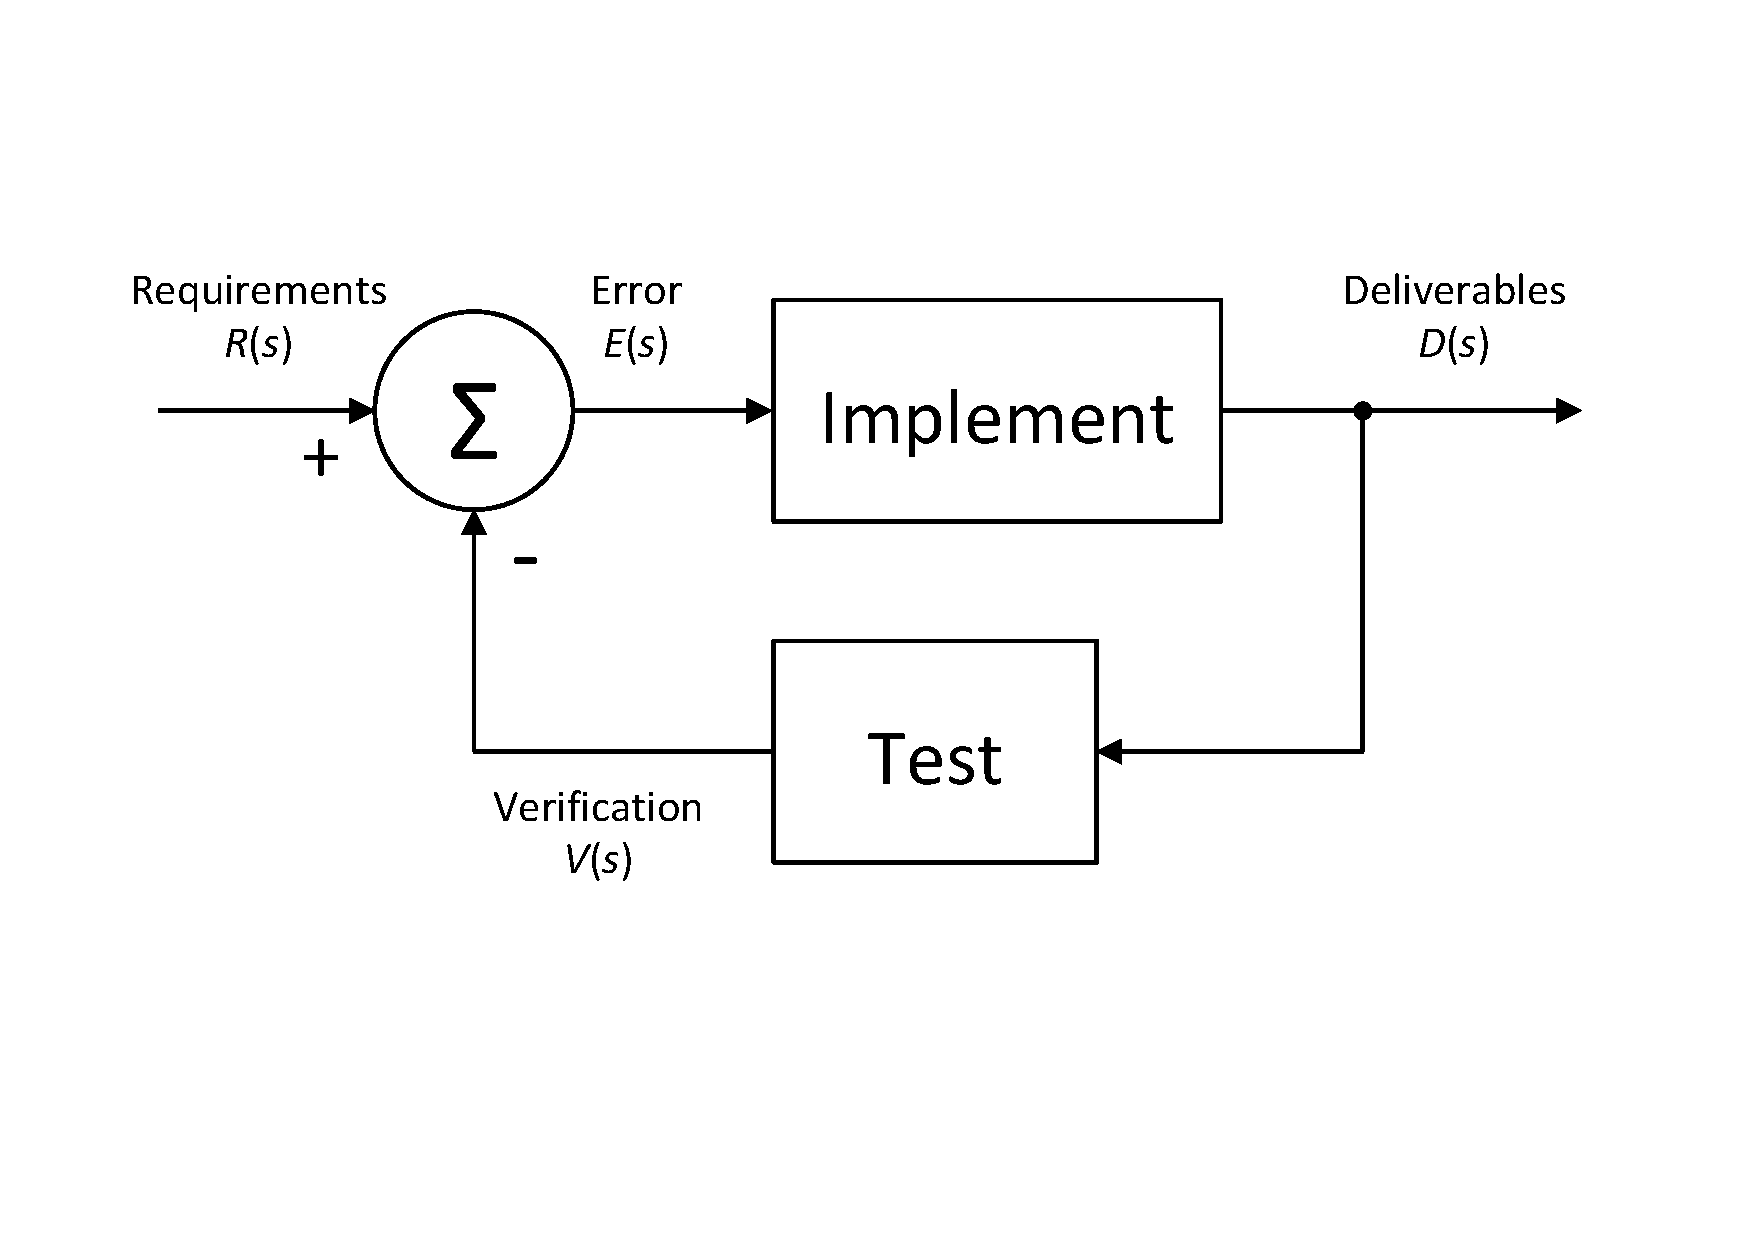
\includegraphics[width=\textwidth]{figures/figure1}
\caption{Software development process rendered as a closed-loop control simulation diagram. Negative feedback from the \textit{Test} block causes the \textit{Deliverables} to evolve, tracking changes in \textit{Requirements}. When all requirements have been met, the error term $E(s)$ goes to zero and the control loop is in steady state.}
\label{closedLoopModel}
\end{figure}

Many models are available for software development for this discussion. Here we present a simple model based on closed loop control theory, which includes concepts of time dependence and iteration. Figure \ref{closedLoopModel} is a simulation diagram representing a software development process. The input on the left is requirements $R(s)$, and the output on the right is executable code and other deliverable assets $D(s)$. In between we have a means for creating code \textit{Implement} positioned as the plant in control theory, and a means for testing code \textit{Test} positioned as the sensor. The summing junction on the left compares test results $V(s)$ with requirements $R(s)$ to produce an error term $E(s)$, which then drives ongoing development. The directed edges connecting these parts together represent $N$-dimensional vectors where $N$ is the number of requirements. The value of each dimension is the extent to which the given requirement has been met on some arbitrary scale.

A typical software project will begin with all vectors pointing to the origin: no requirements, no implementation, and no tests. As development proceeds we add requirements which drive the implementation, which is then tested and compared with requirements. Each directed edge conveys important information, but the most interesting vector is the error term $E(s)$. This will wander in an $N$-dimensional problem space, with $N$ steadily increasing as development proceeds. Ideally this vector should always trend towards zero, with distance from the origin giving us an indication of how far we are from done. Time dependence is not shown explicitly but one can imagine one or more integrators in the loop, with time constants we may or may not control, which modify the time domain response of the development system.

Treating the development process as continuous we can write an expression for deliverables $D(s)$ in terms of implementation $I(s)$, test $T(s)$, and requirements $R(s)$, where $s$ is the Laplace variable.

\begin{equation}
D(s) = R(s)\frac{I(s)}{1+I(s)T(s)}
\label{transferFunction}
\end{equation}


In this model we see that there are three things which matter: requirements, implementation, and tests. These pillars of software development should receive equal priority during development, so that all three can be considered as correct and complete when development ends and maintenance phase begins. As a practical matter however many projects end with one or more pillars incomplete. I claim without proof that given any one of these, the other two can be derived through various means. For the purposes of this paper we use the simulation diagram in figure \ref{closedLoopModel} to define deriving implementation and tests from requirements as ``forward engineering.'' Starting with an implementation or a test suite is then defined as ``reverse engineering.''

\section{Object model for small targets}

Developers of embedded software for small targets may be tempted to organize their object model around things the system has. Such as inputs, outputs, sensors, and actuators. I would submit however that a coherent design is more likely to result from an object model organized around things the embedded system can do. Such as ``home an axis'', ``measure a sample'', ``acquire a trace'', or ``energize a solenoid.'' The only reason we think in terms of objects is so that we can throw them into a container and iterate over them. While there may be a use case for iterating over peripherals, the important use case here is iterating over a collection of nodes which represent actions a user might want to invoke. Packaged along with the arguments needed to carry out each action. Thus we replace a noun-oriented design with a verb-oriented design so that command nodes can be collected into sequences which can then operate on live hardware, simulated hardware, or a hybrid of both. Let's look at an example of how such a design might arise.

Consider a small target with embedded processor and several channels of analog-to-digital (ADC) conversion. On first bring-up we want to start characterizing the ADC input. We write a small monitor program with a command prompt exposed on a serial port, or a socket port if so equipped. Then we write commands to initialize the ADC, trigger a conversion, and report the result. Each of the commands can be followed with one or more arguments giving details such as sample rate and channel selection. Running a terminal program on a host computer allows us to manually exercise various behaviors of the ADC. We can stream a text file containing ADC commands from the host to the target's monitor program to execute a measurement sequence of arbitrary complexity. ADC conversions however take finite time, and we wind up overrunning the monitor program with new commands before old ones are complete. So we write a program to run on the host and carry out a series of ADC measurements on the target using monitor program commands, but now waiting for a new prompt from the target before sending a new command from the host.

Many readers will have gone through these steps in bringing up a new target. We don't yet have a small language, but many of the pieces needed are already in place. Now we implement our object model, starting on the host side, declaring a class object for each command and an instance attribute for each argument the command needs. One can also add an instance attribute for the command's return value, if it makes sense for the particular use case. Now we can write a program on the host side which can interact with live hardware through the monitor command prompt, or with a simulation which emulates the same interface. Now we have a small language we can use to carry out the following steps:

\begin{itemize}
 \item Instantiate one or more class objects on the host representing command nodes to be executed.
 \item Populate the nodes with arguments appropriate for the desired measurements.
 \item Compose the nodes into a program by appending them to a collection on the host.
 \item Iterate over the collection, interpreting each node as a command with arguments to be sent to the target.
 \item Capture the results returned from the target for each command node, either as attributes of the command nodes or in a separate trace or listing.
\end{itemize}

Let's look at what we have. The class objects representing command nodes can live almost anywhere: on the host, on the target, in the cloud, or anywhere else that can interpret them into commands with the desired arguments. For now we think of the arguments as being hard-coded, but they could just as well be derived or symbolic. The type of collection used to iterate over the command nodes doesn't matter much, except that iteration should follow a predictable repeatable path. The commands themselves can be sent to one or more target devices, or to any other device or simulation with an interface to receive them. Command replies (measurement results or error messages in our ADC example) can go back to the host, to some other monitor, or even be ignored. This then is the bare minimum of what's needed to claim we have a small domain-specific language. This can be prototyped and running in a matter of a few days, completely avoiding the trap that ``nothing works until everything works.''

Now let's look at what's missing. To obtain a text representation of the program we'll need a means to serialize the collection of command nodes. We have many well-established choices such as JSON, XML, YAML, etc. We also have the freedom to design our own representation if warranted, or just dispense with source code text if not. In this paper we will assume without loss of generality that JSON has been chosen. Experience shows that it is trivial to add a serialize method to command node classes, which is specialized for specific commands and arguments. Instead of iterating over the collection while executing each node, we iterate over the collection while serializing each node to obtain a program listing. If we have multiple interpreters (host, target, cloud, etc.) all should produce an identical program listing for a given collection of command nodes. It should be mentioned here that while off-target interpreters can use the monitor command prompt interface, on-target interpreters don't have to since they can also call directly into functions on the target.

Real programming implies branching and looping, which is easily added by declaring command nodes for conditional and repeated execution where the arguments represent loop count, limits for comparison, etc. At this point we've only described programs which are a simple list or sequence of nodes, so conditional and repeated execution would only affect nodes which are after the control node in the list. Nested iterations are implemented by appending more than one repeating node to the list. Multiple conditional nodes in a list must evaluate as ``true'' for nodes following them to be reached. Everything we've done up to this point has light weight and a small footprint.

Now we will add a feature which enables scalable portable solutions by generalizing the command list to a composite command tree.  









\end{document}
